\documentclass[11pt]{article}
\usepackage[textwidth=18.0cm, textheight=23.0cm, top=2.0cm]{geometry}
\usepackage{pst-all}
\usepackage{amssymb}
\usepackage{tikz}
\usepackage{underscore}\begin{document}
\pagestyle{empty}


ClassName: \underline{\textbf{Class_07.2bp-26}}
\par
BinSize: \underline{\textbf{100 × 100}}
\par
ReduceSize: \underline{\textbf{100 × 100}}
\par
TypeNum: \underline{\textbf{60}}
\par
Num: \underline{\textbf{60}}
\par
OutS: \underline{\textbf{150000}}
\par
InS: \underline{\textbf{124373}}
\par
Rate: \underline{\textbf{0.829}}
\par
UB: \underline{\textbf{15}}
\par
LB0: \underline{\textbf{15}}
\par
LB: \underline{\textbf{15}}
\par
LBWithCut: \underline{\textbf{15}}
\par
NodeCut: \underline{\textbf{0}}
\par
ExtendedNodeCnt: \underline{\textbf{1}}
\par
GenNodeCnt: \underline{\textbf{1}}
\par
PrimalNode: \underline{\textbf{0}}
\par
ColumnCount: \underline{\textbf{15}}
\par
TotalCutCount: \underline{\textbf{0}}
\par
RootCutCount: \underline{\textbf{0}}
\par
LPSolverCnt: \underline{\textbf{1}}
\par
PricingSolverCnt: \underline{\textbf{0}}
\par
BranchAndBoundNum: \underline{\textbf{1}}
\par
isOpt: \underline{\textbf{true}}
\par
TimeOnInitSolution: \underline{\textbf{600.000 s}}
\par
TimeOnPrimal: \underline{\textbf{0.000 s}}
\par
TimeOnPricing: \underline{\textbf{0.000 s}}
\par
TimeOnRmp: \underline{\textbf{0.062 s}}
\par
TotalTime: \underline{\textbf{600.313 s}}
\par
\newpage


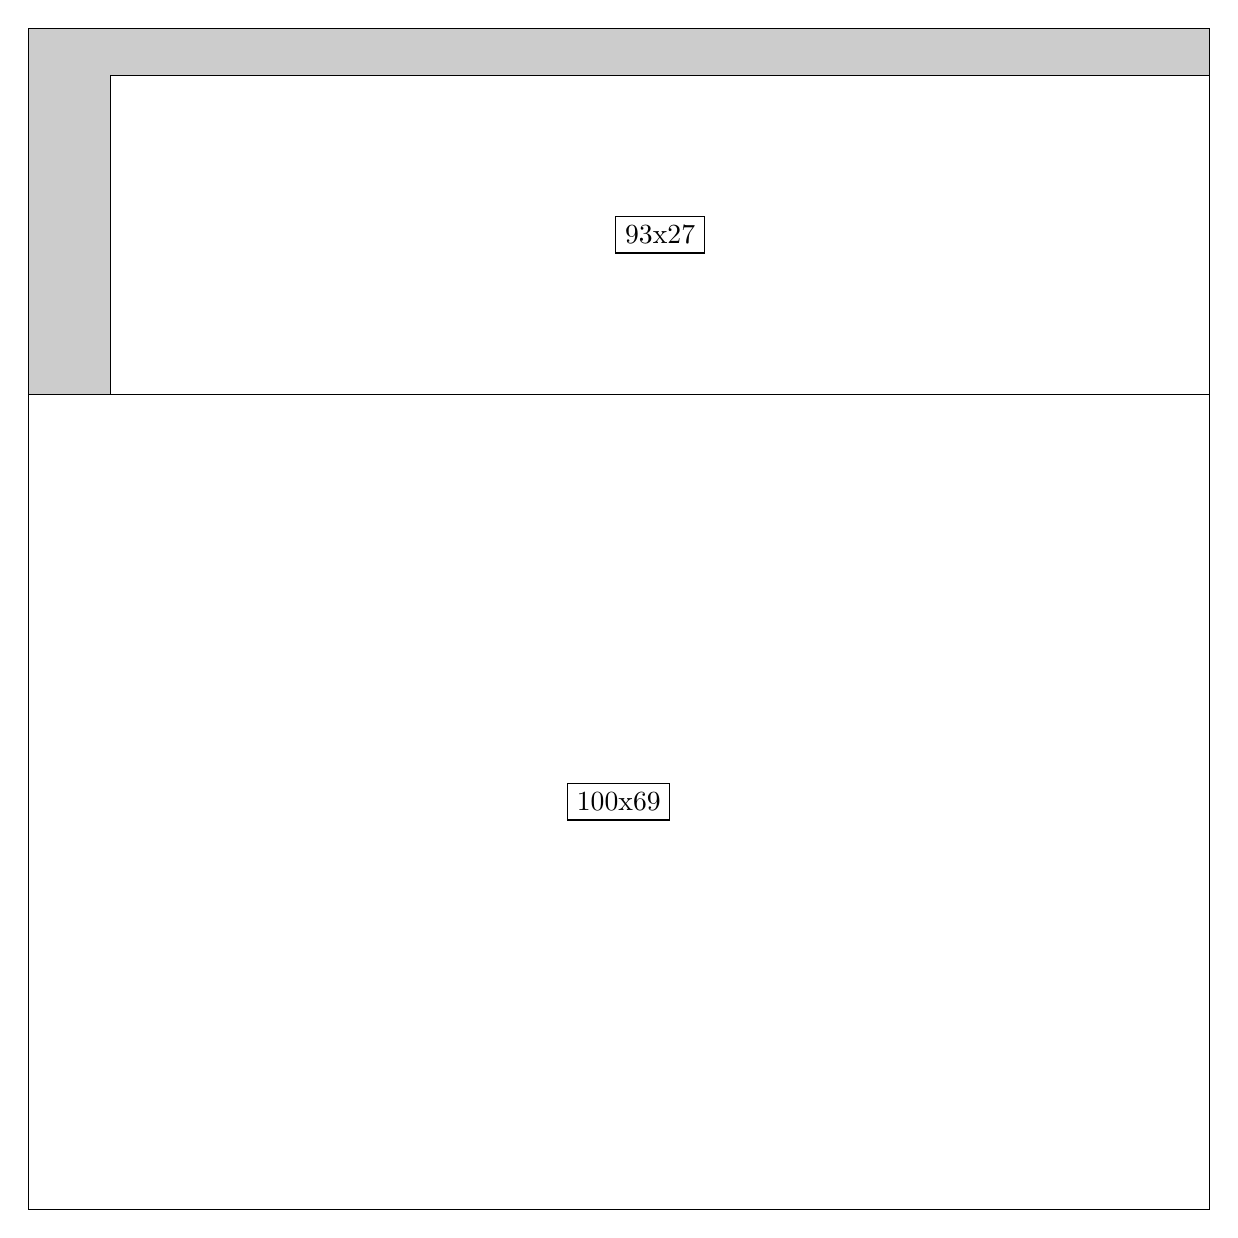
\begin{tikzpicture}[shorten >=1pt,scale=1.0,every node/.style={scale=1.0},->]
\tikzstyle{vertex}=[circle,fill=black!25,minimum size=14pt,inner sep=0pt]
\filldraw[fill=gray!40!white, draw=black] (0,0) rectangle (15.0,15.0);
\foreach \name/\x/\y/\w/\h in {100x69/0.0/0.0/15.0/10.35,93x27/1.05/10.35/13.95/4.05}
\filldraw[fill=white!40!white, draw=black] (\x,\y) rectangle node[draw] (\name) {\name} ++(\w,\h);
\end{tikzpicture}


w =100 , h =69 , x =0 , y =0 , v =6900
\par
w =93 , h =27 , x =7 , y =69 , v =2511
\par
\newpage


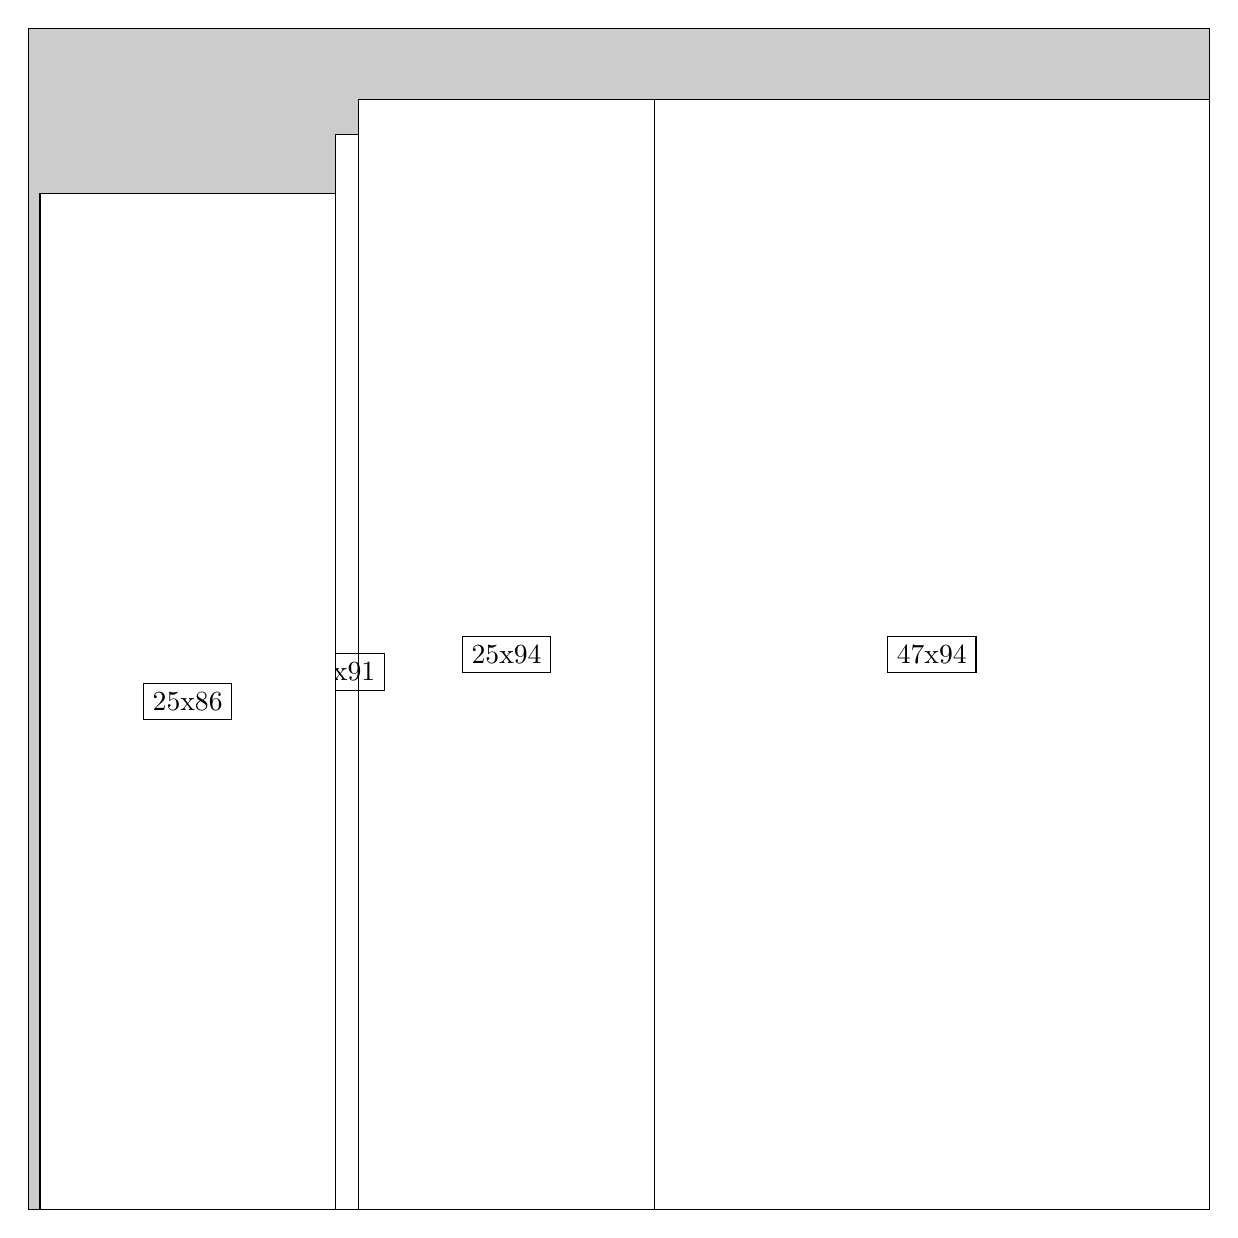
\begin{tikzpicture}[shorten >=1pt,scale=1.0,every node/.style={scale=1.0},->]
\tikzstyle{vertex}=[circle,fill=black!25,minimum size=14pt,inner sep=0pt]
\filldraw[fill=gray!40!white, draw=black] (0,0) rectangle (15.0,15.0);
\foreach \name/\x/\y/\w/\h in {47x94/7.949999999999999/0.0/7.05/14.1,25x94/4.2/0.0/3.75/14.1,2x91/3.9/0.0/0.3/13.65,25x86/0.15/0.0/3.75/12.9}
\filldraw[fill=white!40!white, draw=black] (\x,\y) rectangle node[draw] (\name) {\name} ++(\w,\h);
\end{tikzpicture}


w =47 , h =94 , x =53 , y =0 , v =4418
\par
w =25 , h =94 , x =28 , y =0 , v =2350
\par
w =2 , h =91 , x =26 , y =0 , v =182
\par
w =25 , h =86 , x =1 , y =0 , v =2150
\par
\newpage


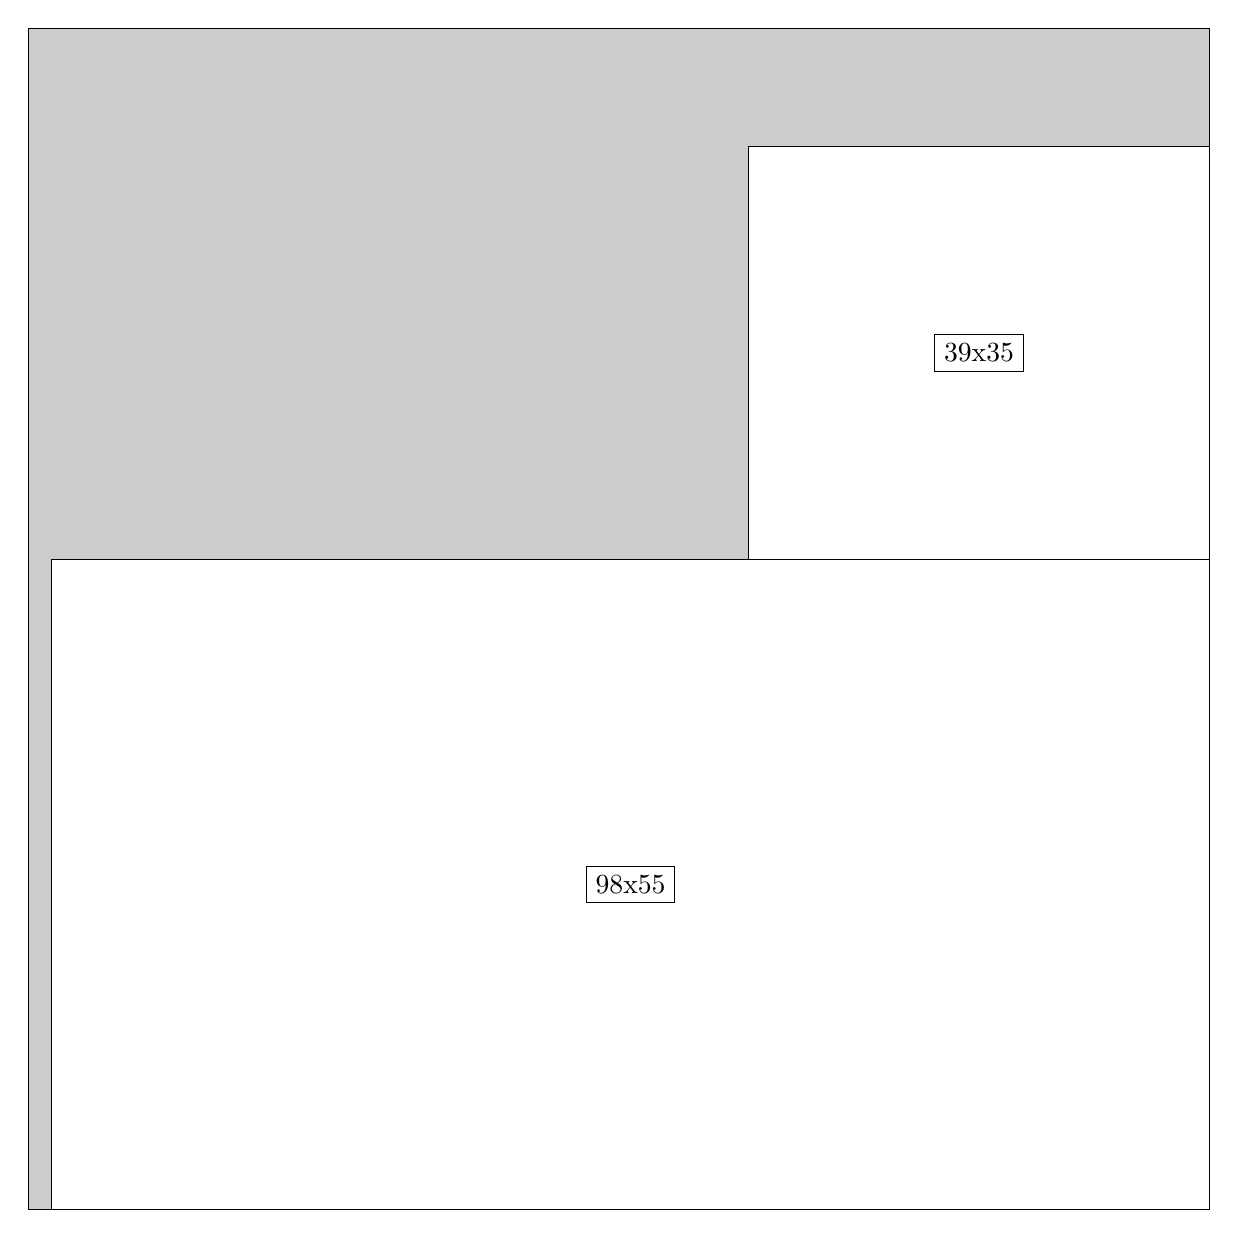
\begin{tikzpicture}[shorten >=1pt,scale=1.0,every node/.style={scale=1.0},->]
\tikzstyle{vertex}=[circle,fill=black!25,minimum size=14pt,inner sep=0pt]
\filldraw[fill=gray!40!white, draw=black] (0,0) rectangle (15.0,15.0);
\foreach \name/\x/\y/\w/\h in {98x55/0.3/0.0/14.7/8.25,39x35/9.15/8.25/5.85/5.25}
\filldraw[fill=white!40!white, draw=black] (\x,\y) rectangle node[draw] (\name) {\name} ++(\w,\h);
\end{tikzpicture}


w =98 , h =55 , x =2 , y =0 , v =5390
\par
w =39 , h =35 , x =61 , y =55 , v =1365
\par
\newpage


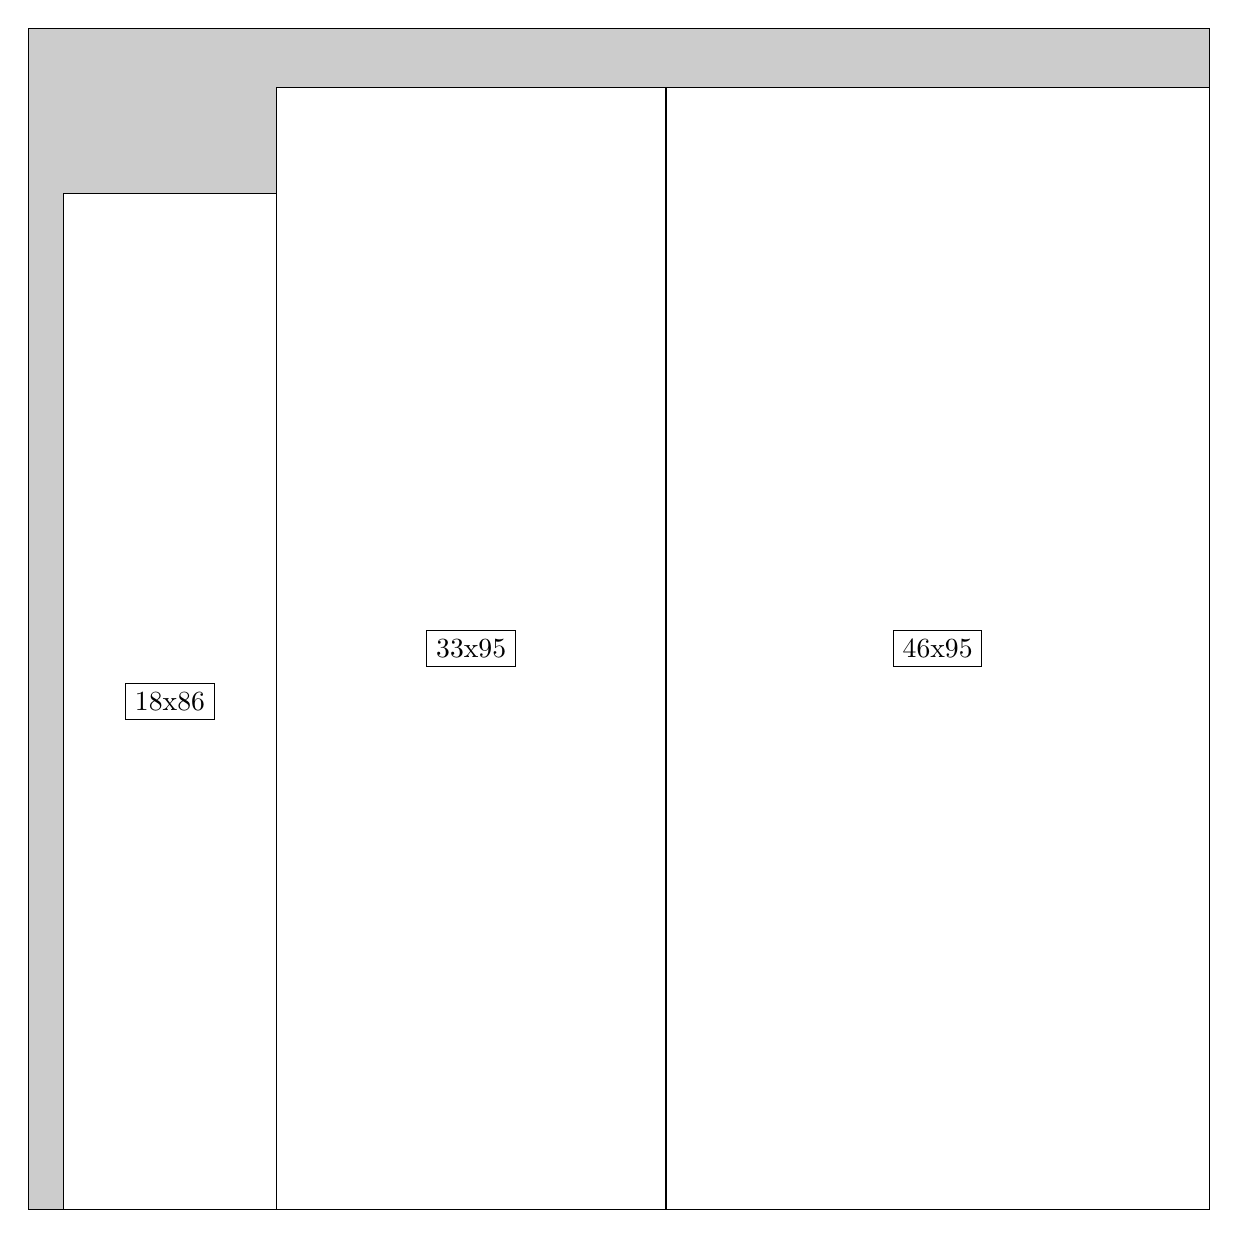
\begin{tikzpicture}[shorten >=1pt,scale=1.0,every node/.style={scale=1.0},->]
\tikzstyle{vertex}=[circle,fill=black!25,minimum size=14pt,inner sep=0pt]
\filldraw[fill=gray!40!white, draw=black] (0,0) rectangle (15.0,15.0);
\foreach \name/\x/\y/\w/\h in {46x95/8.1/0.0/6.8999999999999995/14.25,33x95/3.15/0.0/4.95/14.25,18x86/0.44999999999999996/0.0/2.6999999999999997/12.9}
\filldraw[fill=white!40!white, draw=black] (\x,\y) rectangle node[draw] (\name) {\name} ++(\w,\h);
\end{tikzpicture}


w =46 , h =95 , x =54 , y =0 , v =4370
\par
w =33 , h =95 , x =21 , y =0 , v =3135
\par
w =18 , h =86 , x =3 , y =0 , v =1548
\par
\newpage


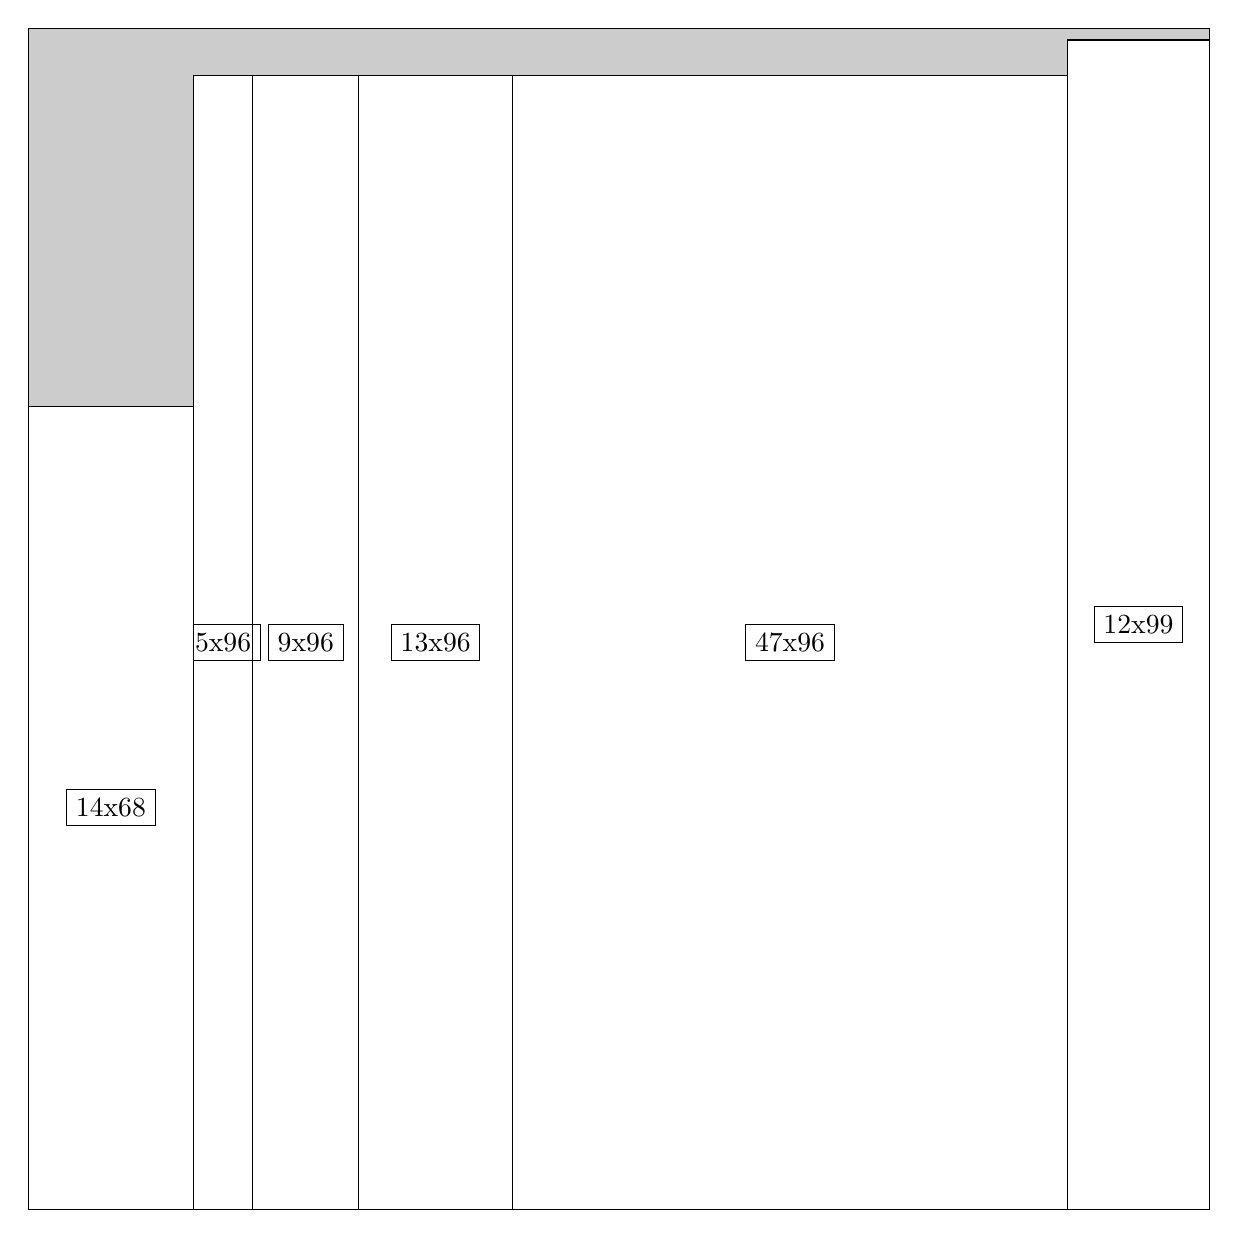
\begin{tikzpicture}[shorten >=1pt,scale=1.0,every node/.style={scale=1.0},->]
\tikzstyle{vertex}=[circle,fill=black!25,minimum size=14pt,inner sep=0pt]
\filldraw[fill=gray!40!white, draw=black] (0,0) rectangle (15.0,15.0);
\foreach \name/\x/\y/\w/\h in {12x99/13.2/0.0/1.7999999999999998/14.85,47x96/6.1499999999999995/0.0/7.05/14.399999999999999,13x96/4.2/0.0/1.95/14.399999999999999,9x96/2.85/0.0/1.3499999999999999/14.399999999999999,5x96/2.1/0.0/0.75/14.399999999999999,14x68/0.0/0.0/2.1/10.2}
\filldraw[fill=white!40!white, draw=black] (\x,\y) rectangle node[draw] (\name) {\name} ++(\w,\h);
\end{tikzpicture}


w =12 , h =99 , x =88 , y =0 , v =1188
\par
w =47 , h =96 , x =41 , y =0 , v =4512
\par
w =13 , h =96 , x =28 , y =0 , v =1248
\par
w =9 , h =96 , x =19 , y =0 , v =864
\par
w =5 , h =96 , x =14 , y =0 , v =480
\par
w =14 , h =68 , x =0 , y =0 , v =952
\par
\newpage


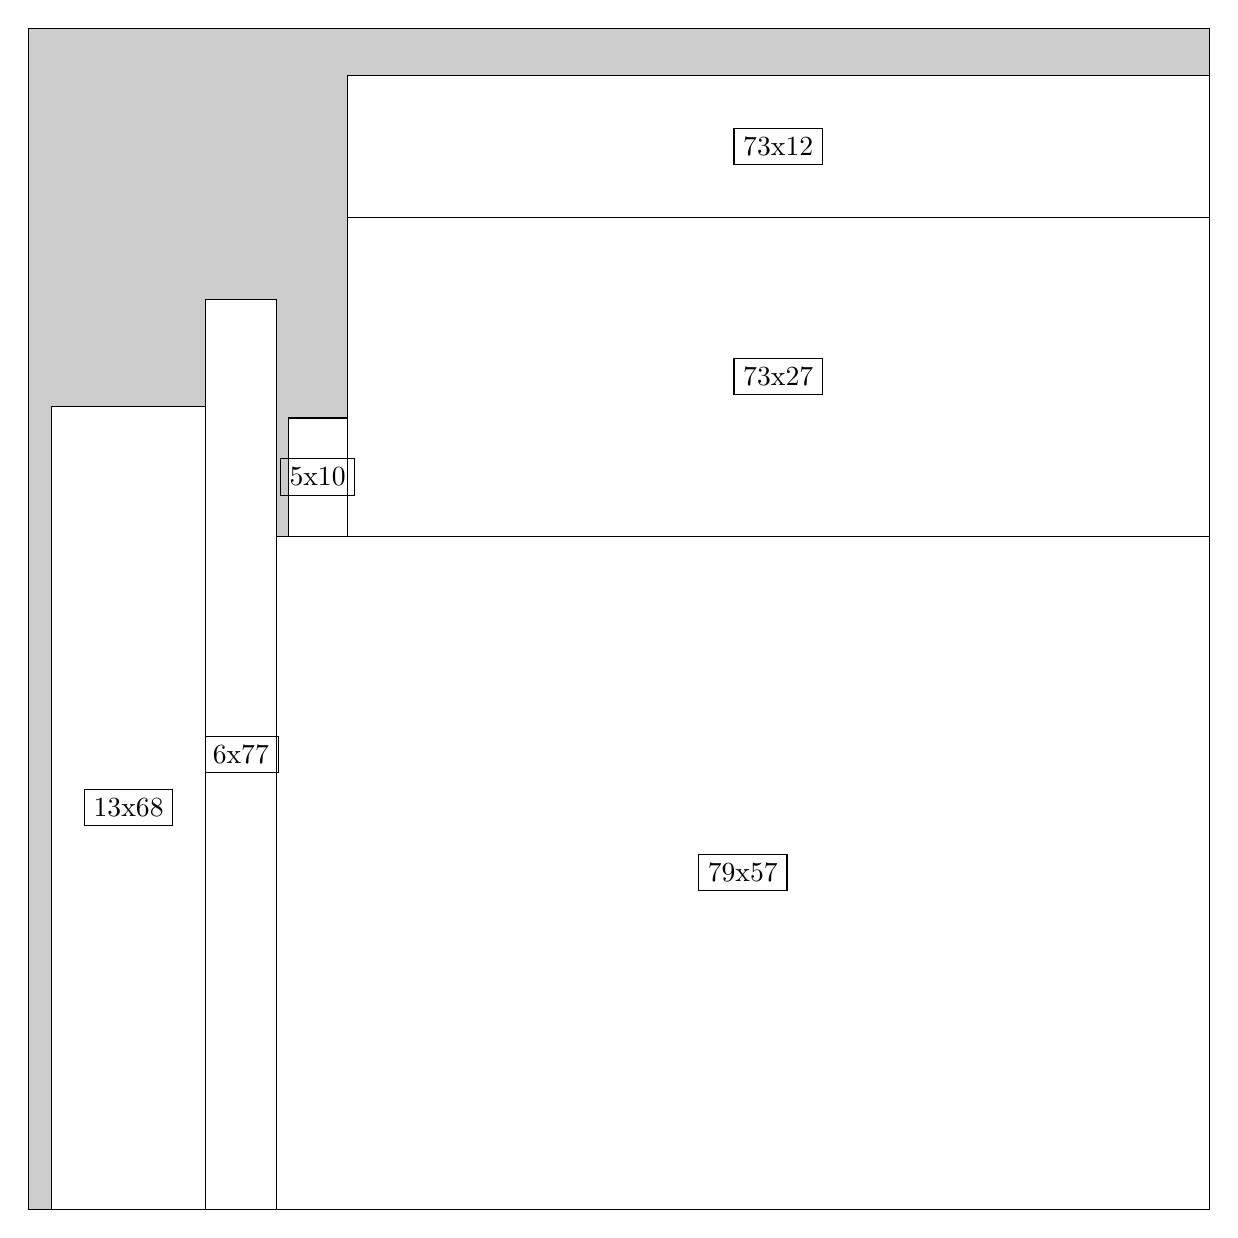
\begin{tikzpicture}[shorten >=1pt,scale=1.0,every node/.style={scale=1.0},->]
\tikzstyle{vertex}=[circle,fill=black!25,minimum size=14pt,inner sep=0pt]
\filldraw[fill=gray!40!white, draw=black] (0,0) rectangle (15.0,15.0);
\foreach \name/\x/\y/\w/\h in {79x57/3.15/0.0/11.85/8.549999999999999,73x27/4.05/8.549999999999999/10.95/4.05,5x10/3.3/8.549999999999999/0.75/1.5,73x12/4.05/12.6/10.95/1.7999999999999998,6x77/2.25/0.0/0.8999999999999999/11.549999999999999,13x68/0.3/0.0/1.95/10.2}
\filldraw[fill=white!40!white, draw=black] (\x,\y) rectangle node[draw] (\name) {\name} ++(\w,\h);
\end{tikzpicture}


w =79 , h =57 , x =21 , y =0 , v =4503
\par
w =73 , h =27 , x =27 , y =57 , v =1971
\par
w =5 , h =10 , x =22 , y =57 , v =50
\par
w =73 , h =12 , x =27 , y =84 , v =876
\par
w =6 , h =77 , x =15 , y =0 , v =462
\par
w =13 , h =68 , x =2 , y =0 , v =884
\par
\newpage


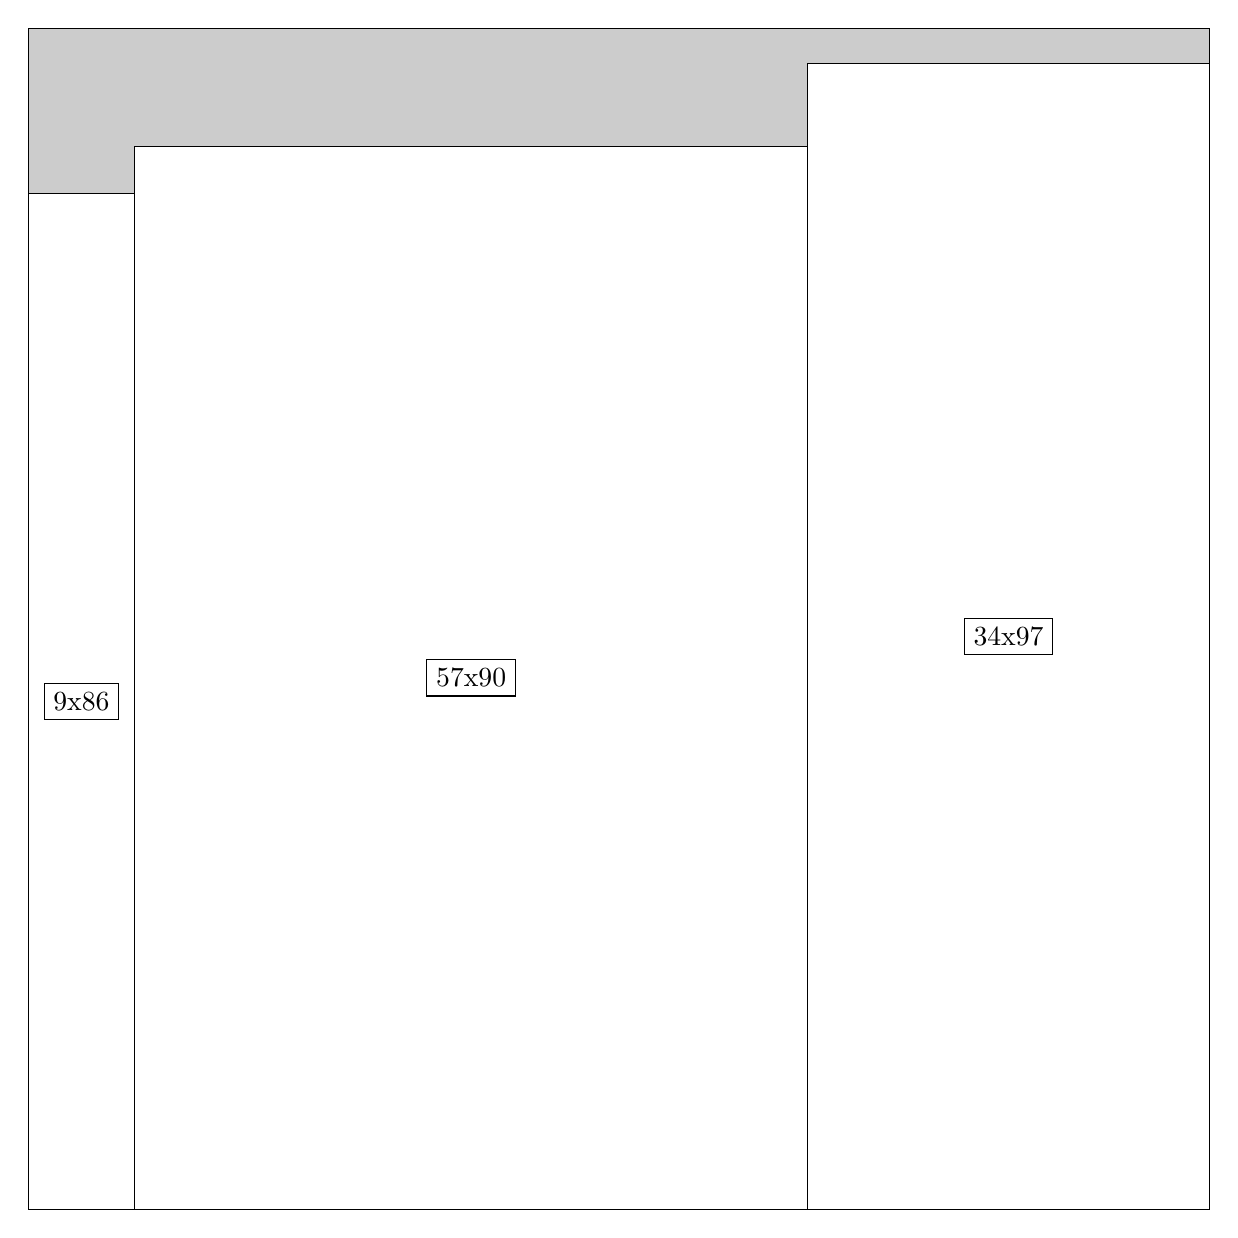
\begin{tikzpicture}[shorten >=1pt,scale=1.0,every node/.style={scale=1.0},->]
\tikzstyle{vertex}=[circle,fill=black!25,minimum size=14pt,inner sep=0pt]
\filldraw[fill=gray!40!white, draw=black] (0,0) rectangle (15.0,15.0);
\foreach \name/\x/\y/\w/\h in {34x97/9.9/0.0/5.1/14.549999999999999,57x90/1.3499999999999999/0.0/8.549999999999999/13.5,9x86/0.0/0.0/1.3499999999999999/12.9}
\filldraw[fill=white!40!white, draw=black] (\x,\y) rectangle node[draw] (\name) {\name} ++(\w,\h);
\end{tikzpicture}


w =34 , h =97 , x =66 , y =0 , v =3298
\par
w =57 , h =90 , x =9 , y =0 , v =5130
\par
w =9 , h =86 , x =0 , y =0 , v =774
\par
\newpage


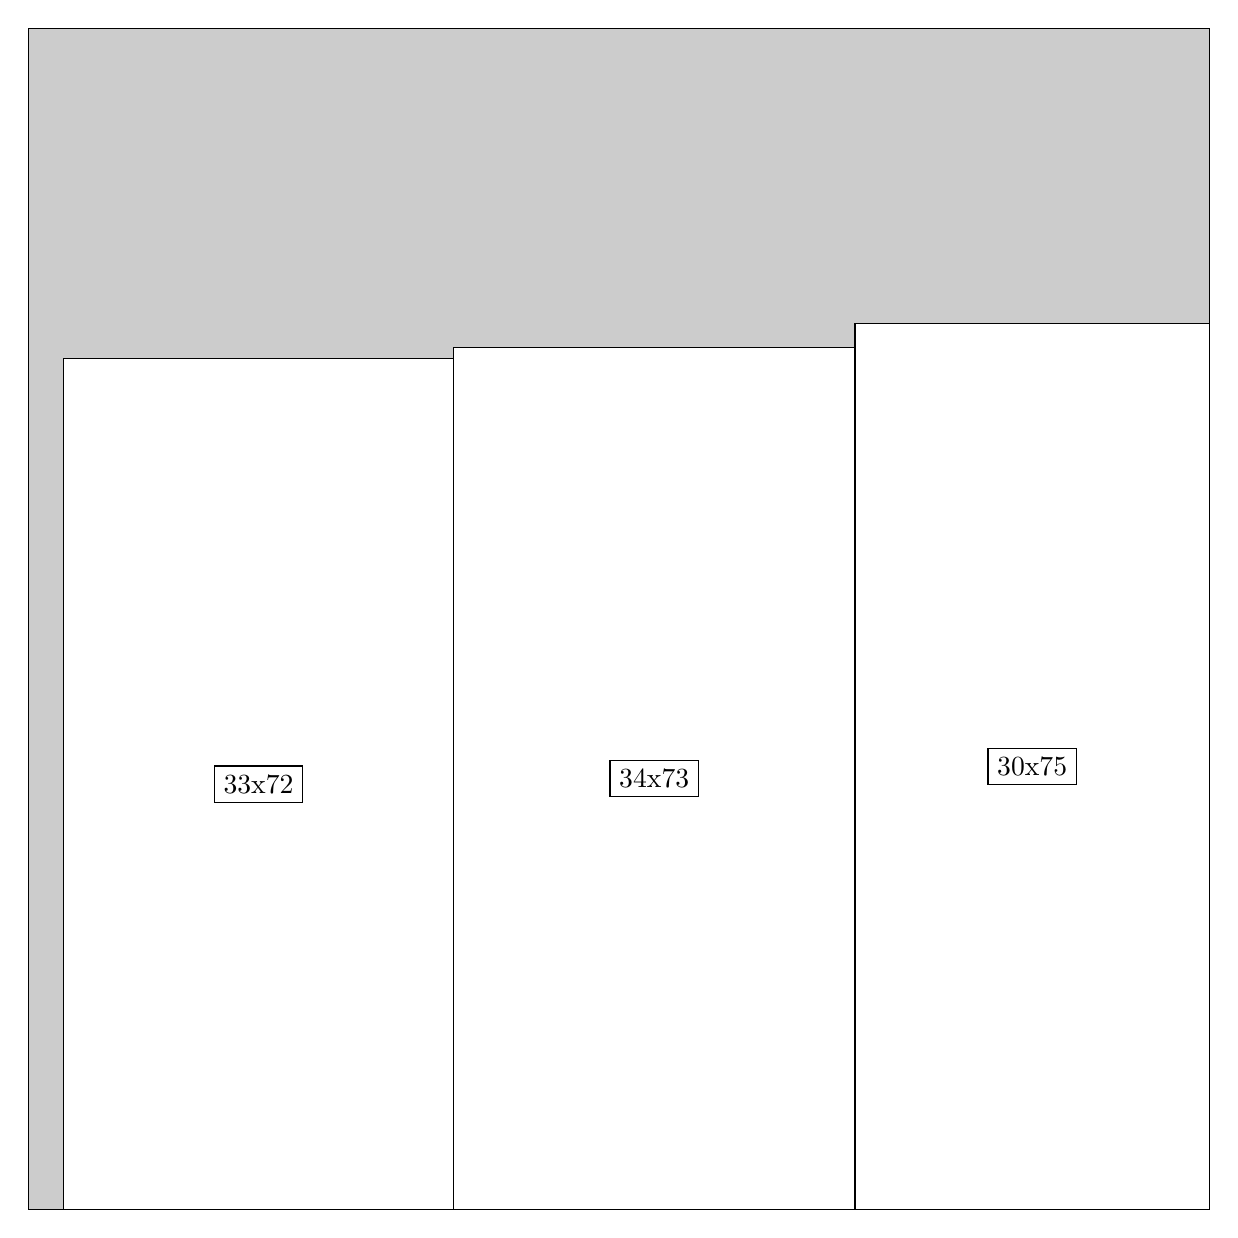
\begin{tikzpicture}[shorten >=1pt,scale=1.0,every node/.style={scale=1.0},->]
\tikzstyle{vertex}=[circle,fill=black!25,minimum size=14pt,inner sep=0pt]
\filldraw[fill=gray!40!white, draw=black] (0,0) rectangle (15.0,15.0);
\foreach \name/\x/\y/\w/\h in {30x75/10.5/0.0/4.5/11.25,34x73/5.3999999999999995/0.0/5.1/10.95,33x72/0.44999999999999996/0.0/4.95/10.799999999999999}
\filldraw[fill=white!40!white, draw=black] (\x,\y) rectangle node[draw] (\name) {\name} ++(\w,\h);
\end{tikzpicture}


w =30 , h =75 , x =70 , y =0 , v =2250
\par
w =34 , h =73 , x =36 , y =0 , v =2482
\par
w =33 , h =72 , x =3 , y =0 , v =2376
\par
\newpage


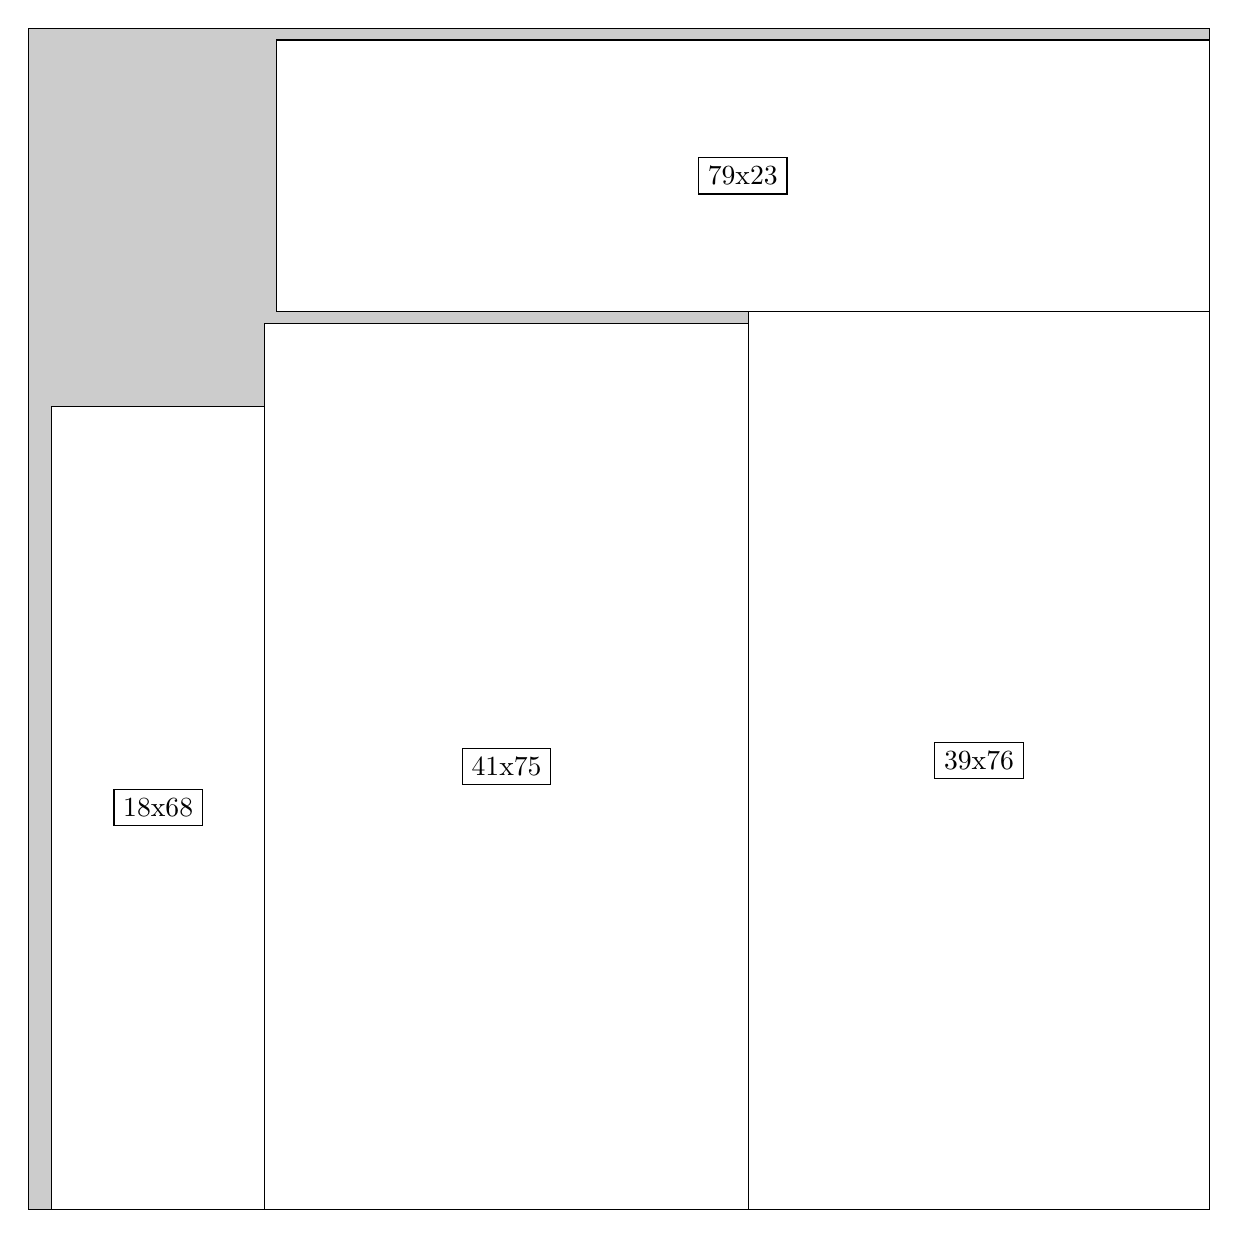
\begin{tikzpicture}[shorten >=1pt,scale=1.0,every node/.style={scale=1.0},->]
\tikzstyle{vertex}=[circle,fill=black!25,minimum size=14pt,inner sep=0pt]
\filldraw[fill=gray!40!white, draw=black] (0,0) rectangle (15.0,15.0);
\foreach \name/\x/\y/\w/\h in {39x76/9.15/0.0/5.85/11.4,41x75/3.0/0.0/6.1499999999999995/11.25,18x68/0.3/0.0/2.6999999999999997/10.2,79x23/3.15/11.4/11.85/3.4499999999999997}
\filldraw[fill=white!40!white, draw=black] (\x,\y) rectangle node[draw] (\name) {\name} ++(\w,\h);
\end{tikzpicture}


w =39 , h =76 , x =61 , y =0 , v =2964
\par
w =41 , h =75 , x =20 , y =0 , v =3075
\par
w =18 , h =68 , x =2 , y =0 , v =1224
\par
w =79 , h =23 , x =21 , y =76 , v =1817
\par
\newpage


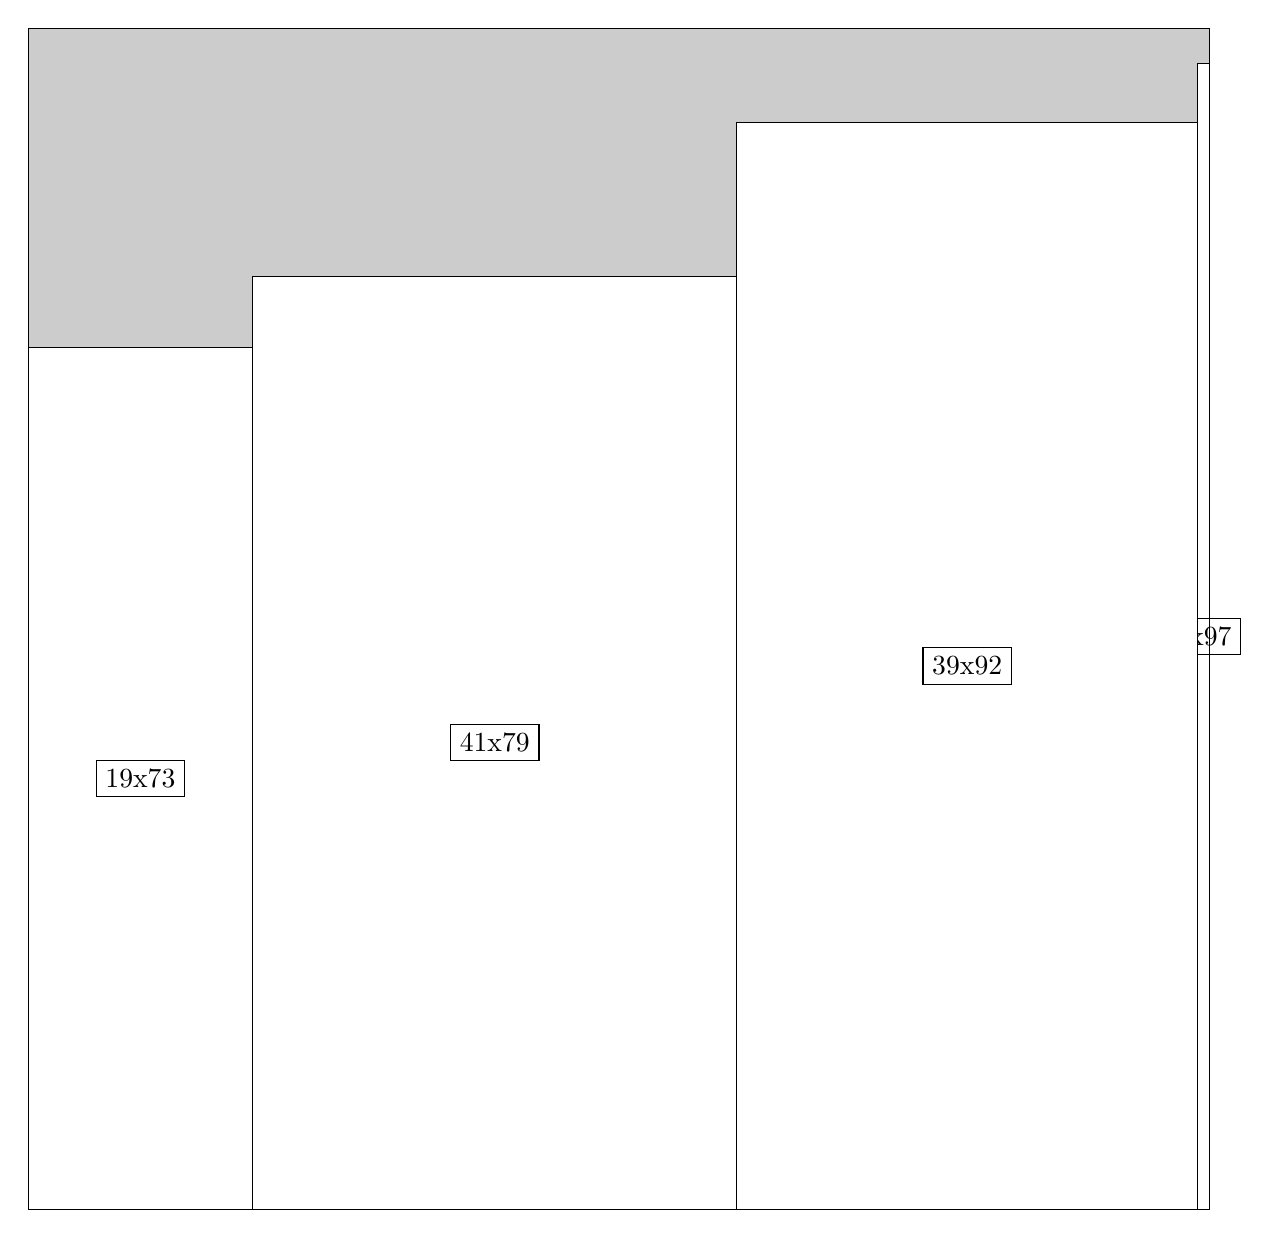
\begin{tikzpicture}[shorten >=1pt,scale=1.0,every node/.style={scale=1.0},->]
\tikzstyle{vertex}=[circle,fill=black!25,minimum size=14pt,inner sep=0pt]
\filldraw[fill=gray!40!white, draw=black] (0,0) rectangle (15.0,15.0);
\foreach \name/\x/\y/\w/\h in {1x97/14.85/0.0/0.15/14.549999999999999,39x92/9.0/0.0/5.85/13.799999999999999,41x79/2.85/0.0/6.1499999999999995/11.85,19x73/0.0/0.0/2.85/10.95}
\filldraw[fill=white!40!white, draw=black] (\x,\y) rectangle node[draw] (\name) {\name} ++(\w,\h);
\end{tikzpicture}


w =1 , h =97 , x =99 , y =0 , v =97
\par
w =39 , h =92 , x =60 , y =0 , v =3588
\par
w =41 , h =79 , x =19 , y =0 , v =3239
\par
w =19 , h =73 , x =0 , y =0 , v =1387
\par
\newpage


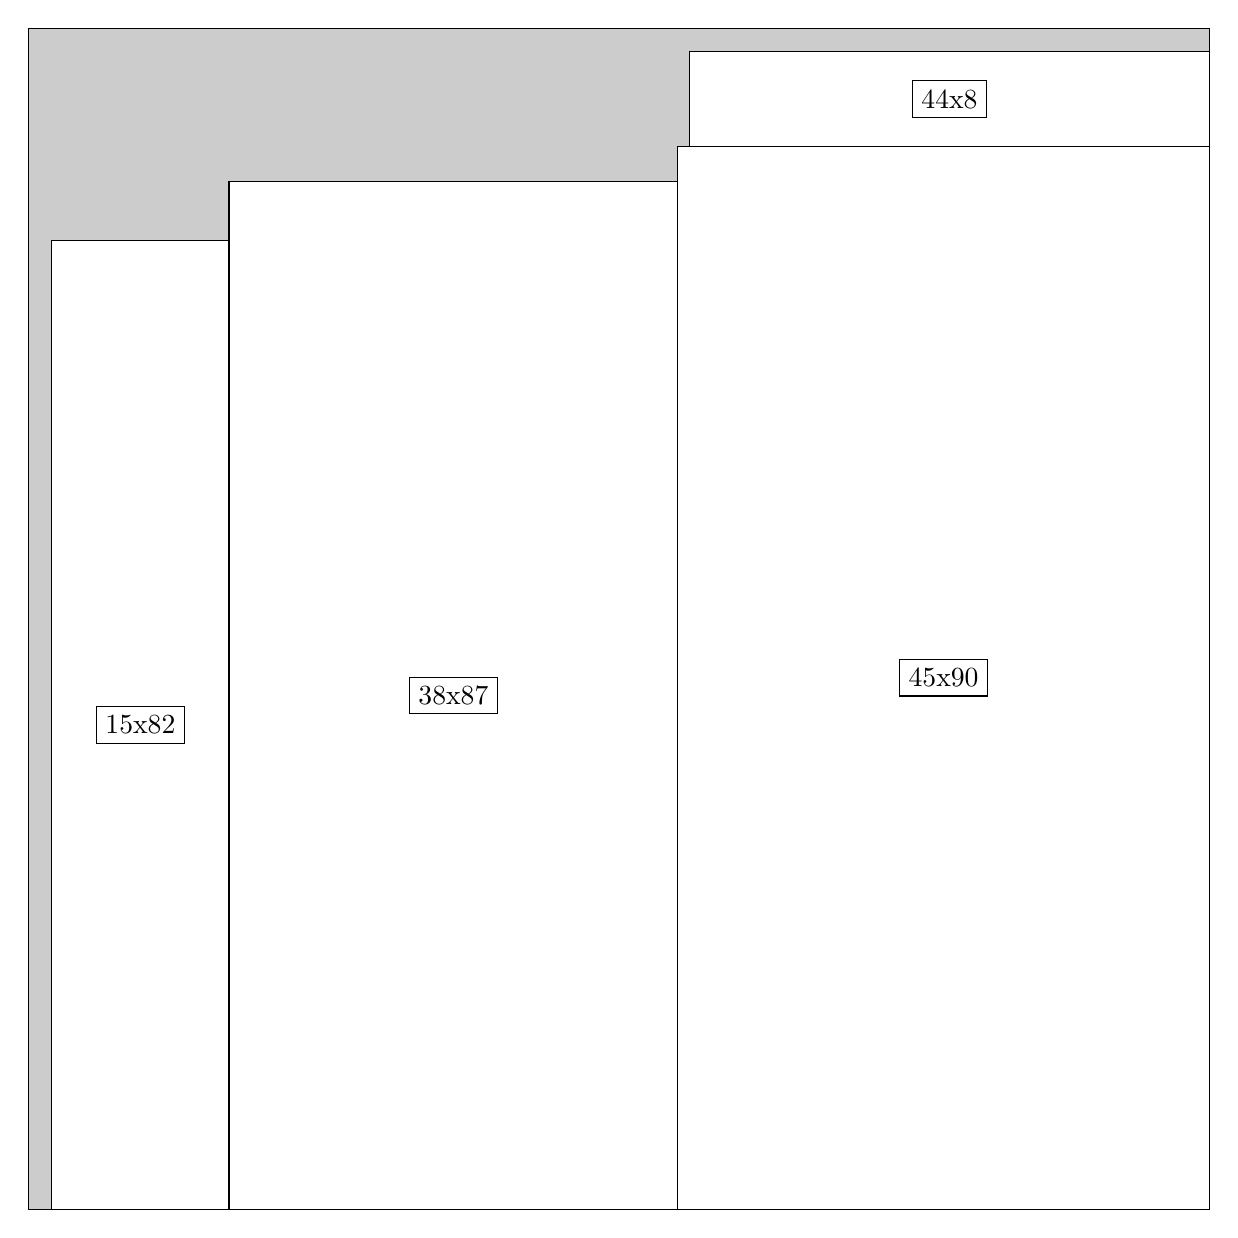
\begin{tikzpicture}[shorten >=1pt,scale=1.0,every node/.style={scale=1.0},->]
\tikzstyle{vertex}=[circle,fill=black!25,minimum size=14pt,inner sep=0pt]
\filldraw[fill=gray!40!white, draw=black] (0,0) rectangle (15.0,15.0);
\foreach \name/\x/\y/\w/\h in {45x90/8.25/0.0/6.75/13.5,44x8/8.4/13.5/6.6/1.2,38x87/2.55/0.0/5.7/13.049999999999999,15x82/0.3/0.0/2.25/12.299999999999999}
\filldraw[fill=white!40!white, draw=black] (\x,\y) rectangle node[draw] (\name) {\name} ++(\w,\h);
\end{tikzpicture}


w =45 , h =90 , x =55 , y =0 , v =4050
\par
w =44 , h =8 , x =56 , y =90 , v =352
\par
w =38 , h =87 , x =17 , y =0 , v =3306
\par
w =15 , h =82 , x =2 , y =0 , v =1230
\par
\newpage


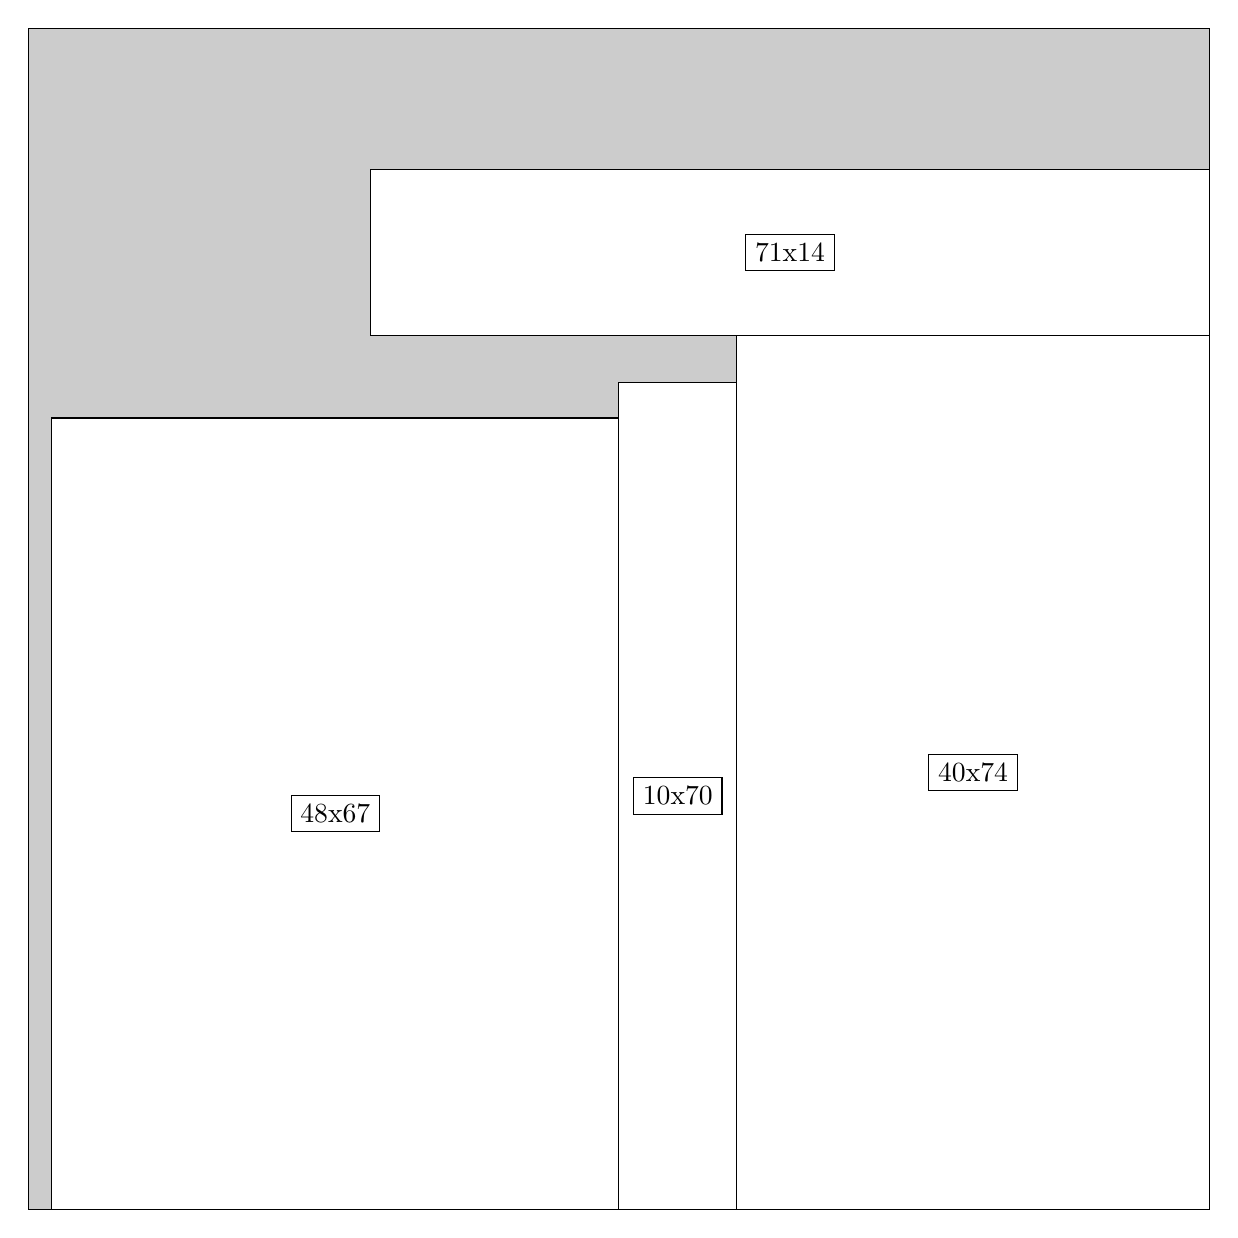
\begin{tikzpicture}[shorten >=1pt,scale=1.0,every node/.style={scale=1.0},->]
\tikzstyle{vertex}=[circle,fill=black!25,minimum size=14pt,inner sep=0pt]
\filldraw[fill=gray!40!white, draw=black] (0,0) rectangle (15.0,15.0);
\foreach \name/\x/\y/\w/\h in {40x74/9.0/0.0/6.0/11.1,10x70/7.5/0.0/1.5/10.5,48x67/0.3/0.0/7.199999999999999/10.049999999999999,71x14/4.35/11.1/10.65/2.1}
\filldraw[fill=white!40!white, draw=black] (\x,\y) rectangle node[draw] (\name) {\name} ++(\w,\h);
\end{tikzpicture}


w =40 , h =74 , x =60 , y =0 , v =2960
\par
w =10 , h =70 , x =50 , y =0 , v =700
\par
w =48 , h =67 , x =2 , y =0 , v =3216
\par
w =71 , h =14 , x =29 , y =74 , v =994
\par
\newpage


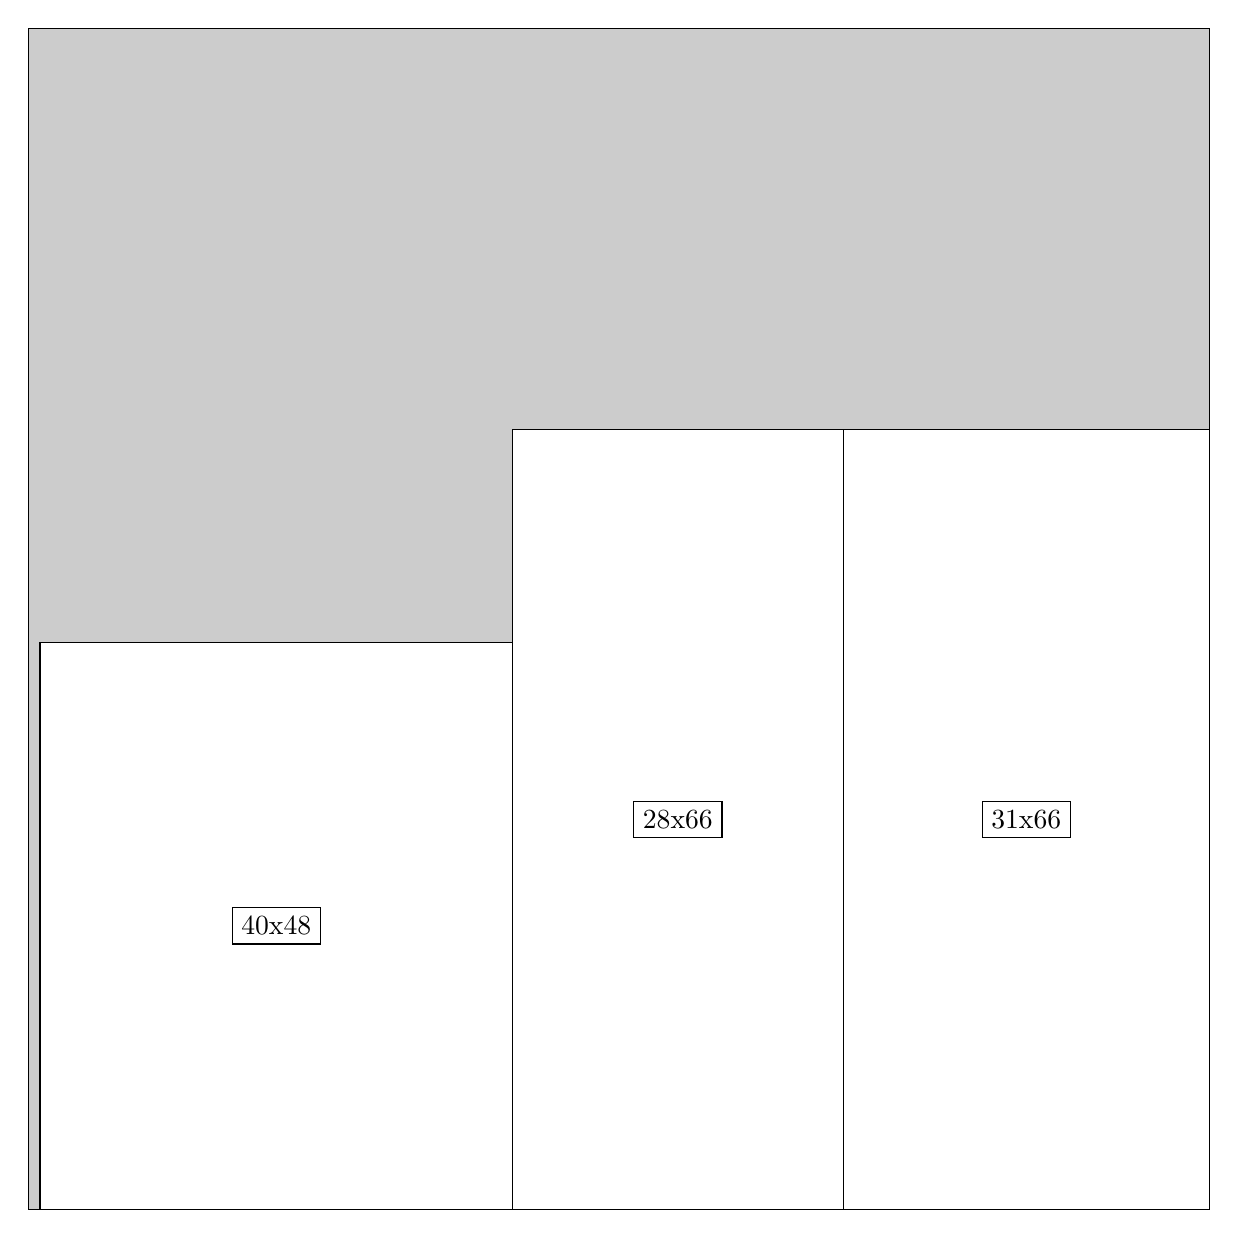
\begin{tikzpicture}[shorten >=1pt,scale=1.0,every node/.style={scale=1.0},->]
\tikzstyle{vertex}=[circle,fill=black!25,minimum size=14pt,inner sep=0pt]
\filldraw[fill=gray!40!white, draw=black] (0,0) rectangle (15.0,15.0);
\foreach \name/\x/\y/\w/\h in {31x66/10.35/0.0/4.6499999999999995/9.9,28x66/6.1499999999999995/0.0/4.2/9.9,40x48/0.15/0.0/6.0/7.199999999999999}
\filldraw[fill=white!40!white, draw=black] (\x,\y) rectangle node[draw] (\name) {\name} ++(\w,\h);
\end{tikzpicture}


w =31 , h =66 , x =69 , y =0 , v =2046
\par
w =28 , h =66 , x =41 , y =0 , v =1848
\par
w =40 , h =48 , x =1 , y =0 , v =1920
\par
\newpage


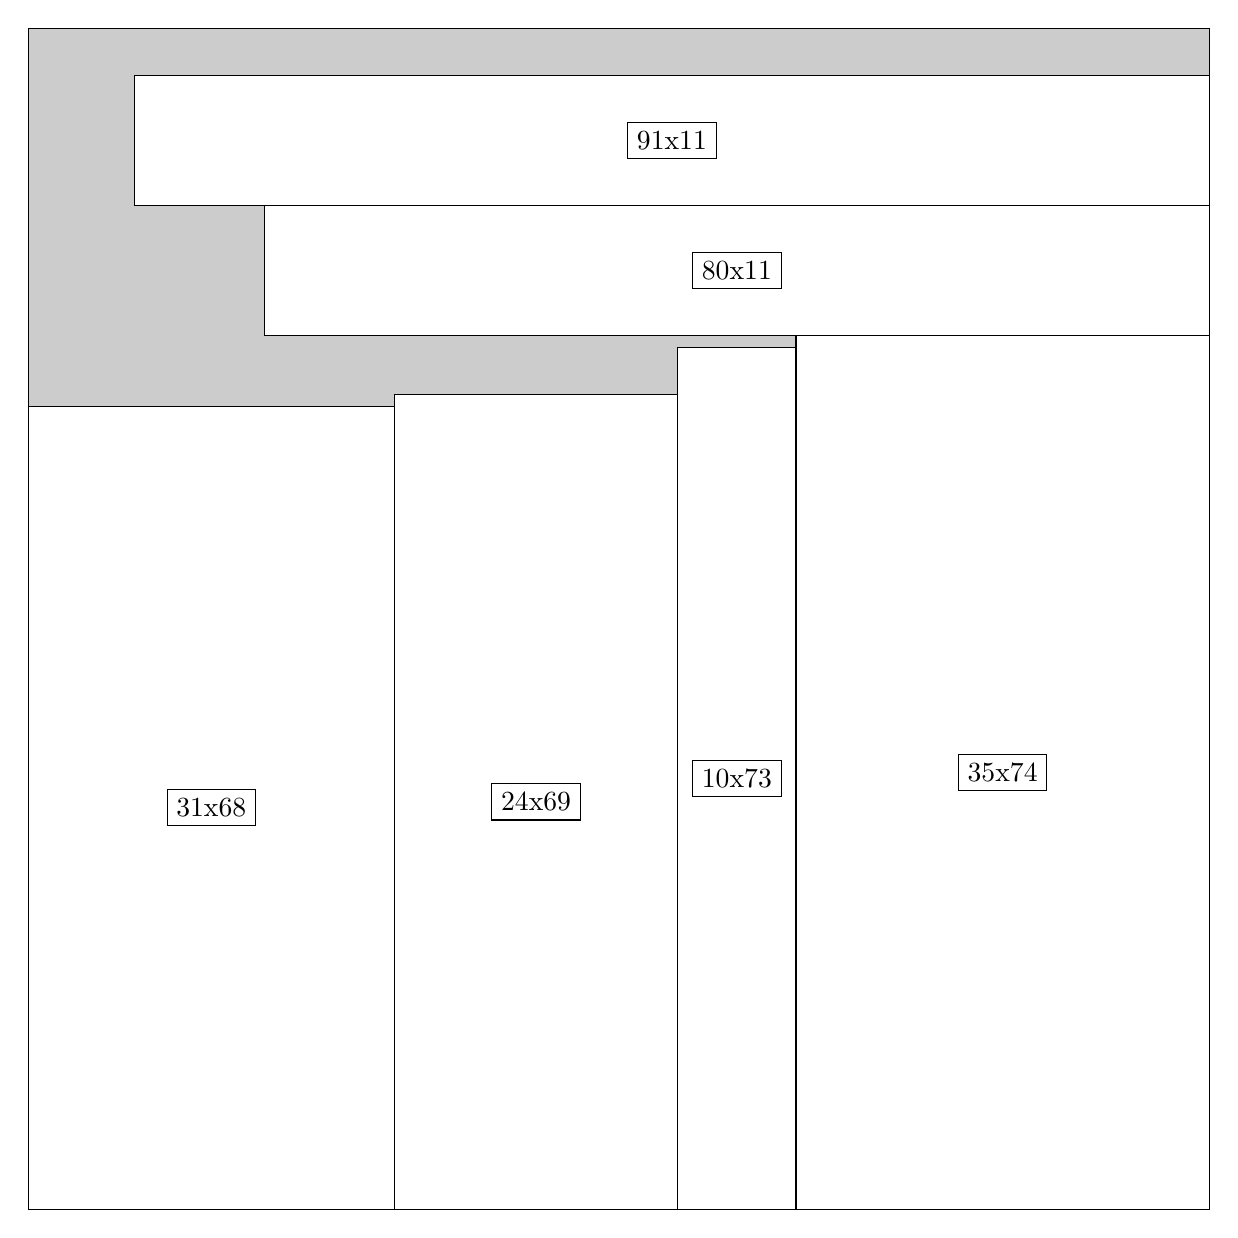
\begin{tikzpicture}[shorten >=1pt,scale=1.0,every node/.style={scale=1.0},->]
\tikzstyle{vertex}=[circle,fill=black!25,minimum size=14pt,inner sep=0pt]
\filldraw[fill=gray!40!white, draw=black] (0,0) rectangle (15.0,15.0);
\foreach \name/\x/\y/\w/\h in {35x74/9.75/0.0/5.25/11.1,10x73/8.25/0.0/1.5/10.95,24x69/4.6499999999999995/0.0/3.5999999999999996/10.35,31x68/0.0/0.0/4.6499999999999995/10.2,80x11/3.0/11.1/12.0/1.65,91x11/1.3499999999999999/12.75/13.65/1.65}
\filldraw[fill=white!40!white, draw=black] (\x,\y) rectangle node[draw] (\name) {\name} ++(\w,\h);
\end{tikzpicture}


w =35 , h =74 , x =65 , y =0 , v =2590
\par
w =10 , h =73 , x =55 , y =0 , v =730
\par
w =24 , h =69 , x =31 , y =0 , v =1656
\par
w =31 , h =68 , x =0 , y =0 , v =2108
\par
w =80 , h =11 , x =20 , y =74 , v =880
\par
w =91 , h =11 , x =9 , y =85 , v =1001
\par
\newpage


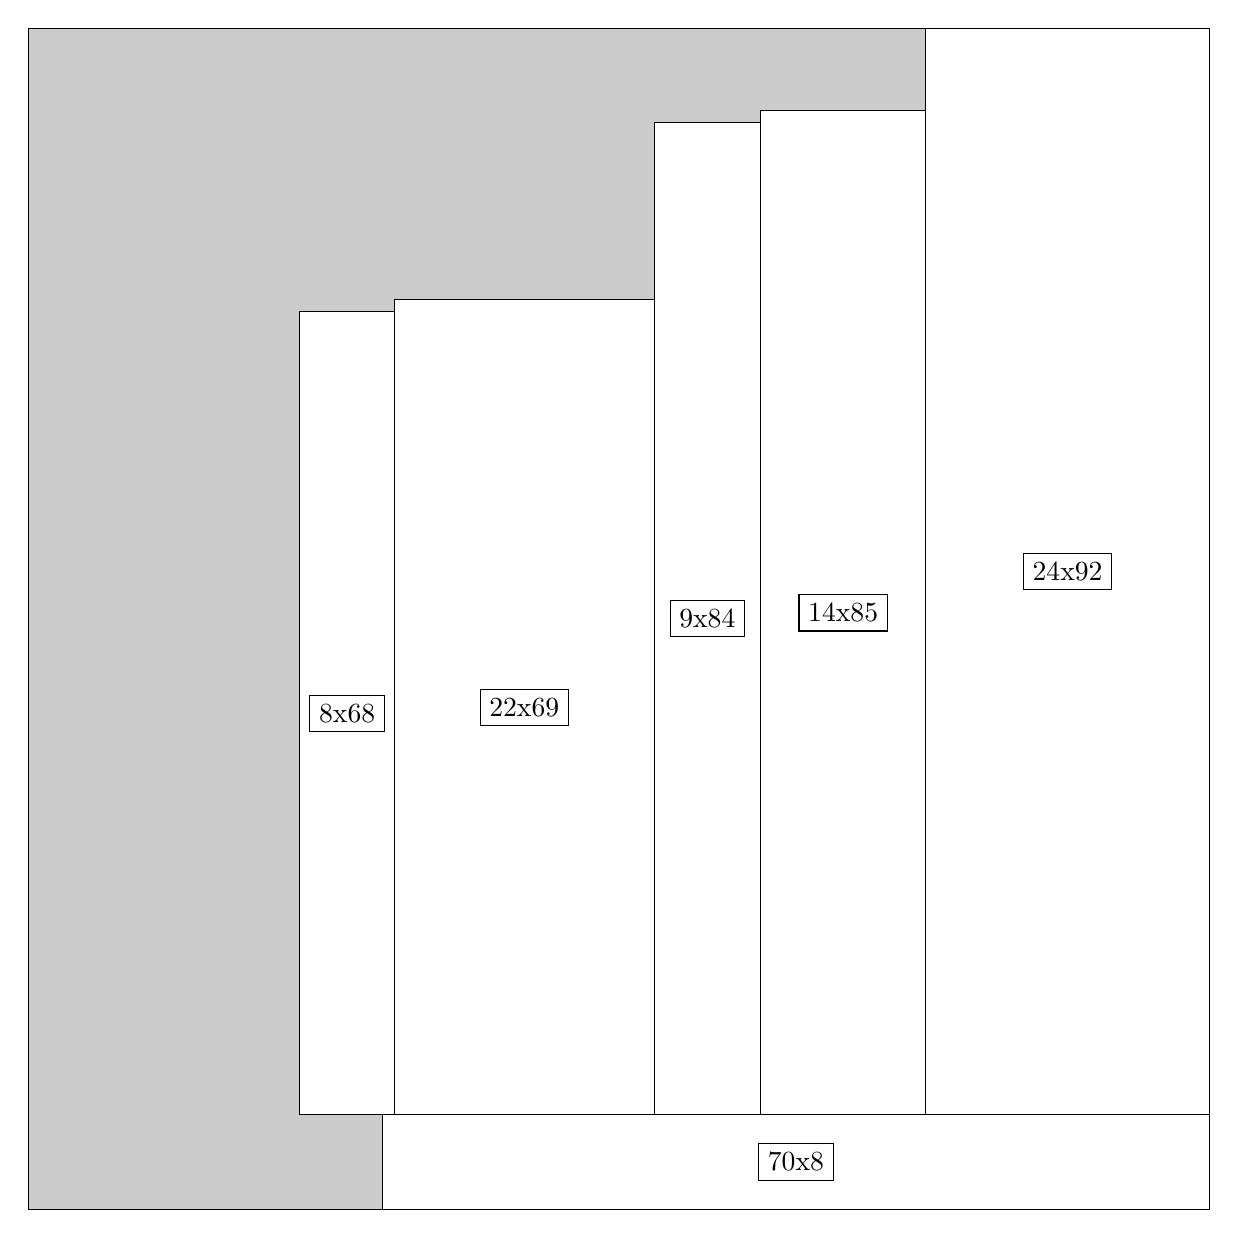
\begin{tikzpicture}[shorten >=1pt,scale=1.0,every node/.style={scale=1.0},->]
\tikzstyle{vertex}=[circle,fill=black!25,minimum size=14pt,inner sep=0pt]
\filldraw[fill=gray!40!white, draw=black] (0,0) rectangle (15.0,15.0);
\foreach \name/\x/\y/\w/\h in {70x8/4.5/0.0/10.5/1.2,24x92/11.4/1.2/3.5999999999999996/13.799999999999999,14x85/9.299999999999999/1.2/2.1/12.75,9x84/7.949999999999999/1.2/1.3499999999999999/12.6,22x69/4.6499999999999995/1.2/3.3/10.35,8x68/3.4499999999999997/1.2/1.2/10.2}
\filldraw[fill=white!40!white, draw=black] (\x,\y) rectangle node[draw] (\name) {\name} ++(\w,\h);
\end{tikzpicture}


w =70 , h =8 , x =30 , y =0 , v =560
\par
w =24 , h =92 , x =76 , y =8 , v =2208
\par
w =14 , h =85 , x =62 , y =8 , v =1190
\par
w =9 , h =84 , x =53 , y =8 , v =756
\par
w =22 , h =69 , x =31 , y =8 , v =1518
\par
w =8 , h =68 , x =23 , y =8 , v =544
\par
\newpage


\end{document}